\section{模范畴}

参见 Rotman: Part I. Chap B-4.

\subsection{Disjoint Union (coProduct) and Product}

\begin{figure}[H]
\centering
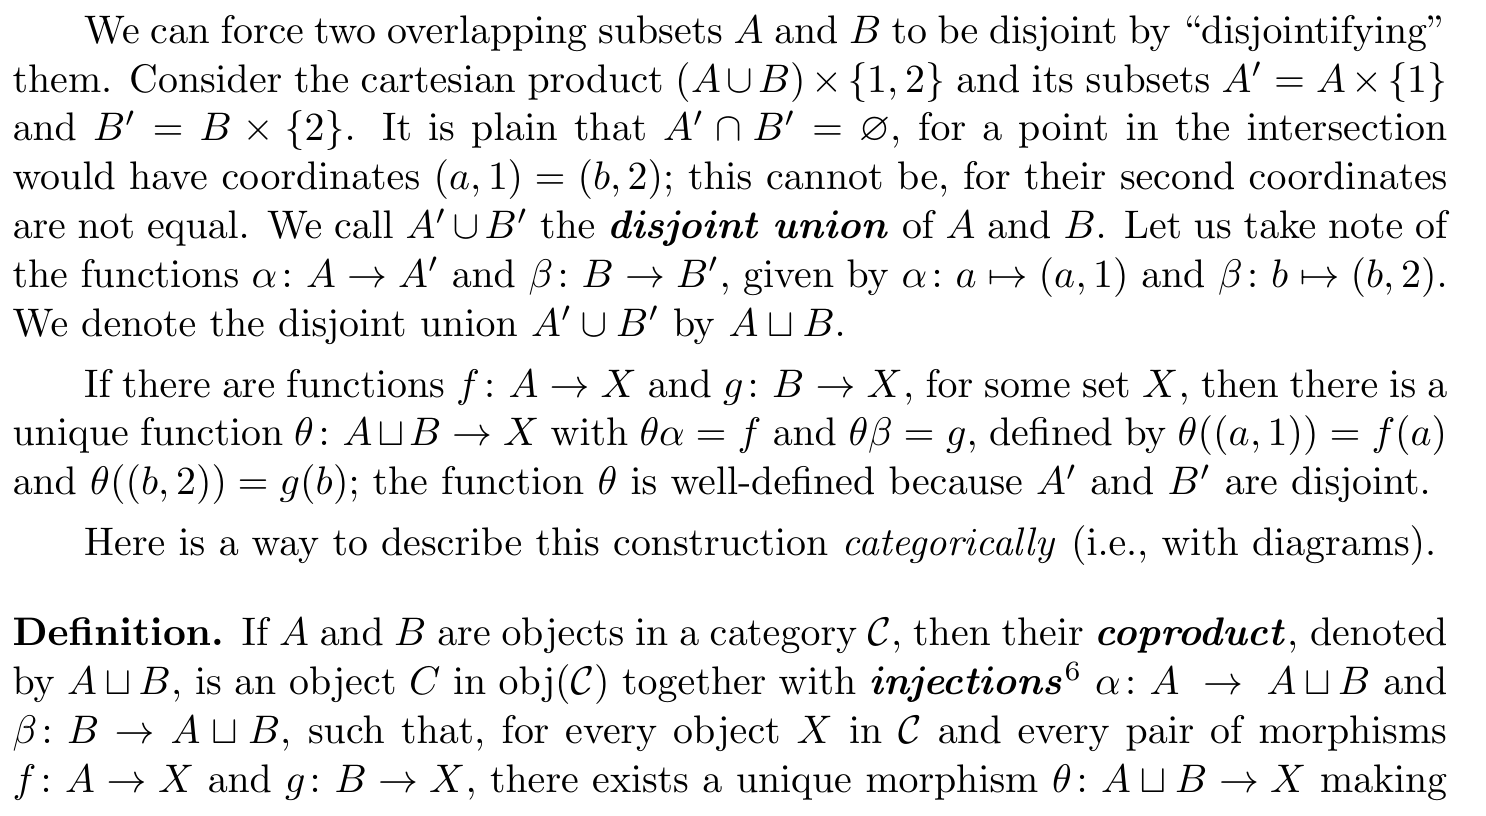
\includegraphics[width=\textwidth]{模范畴-2025052320.png}
% \caption{}
\label{}
\end{figure}

\begin{figure}[H]
\centering
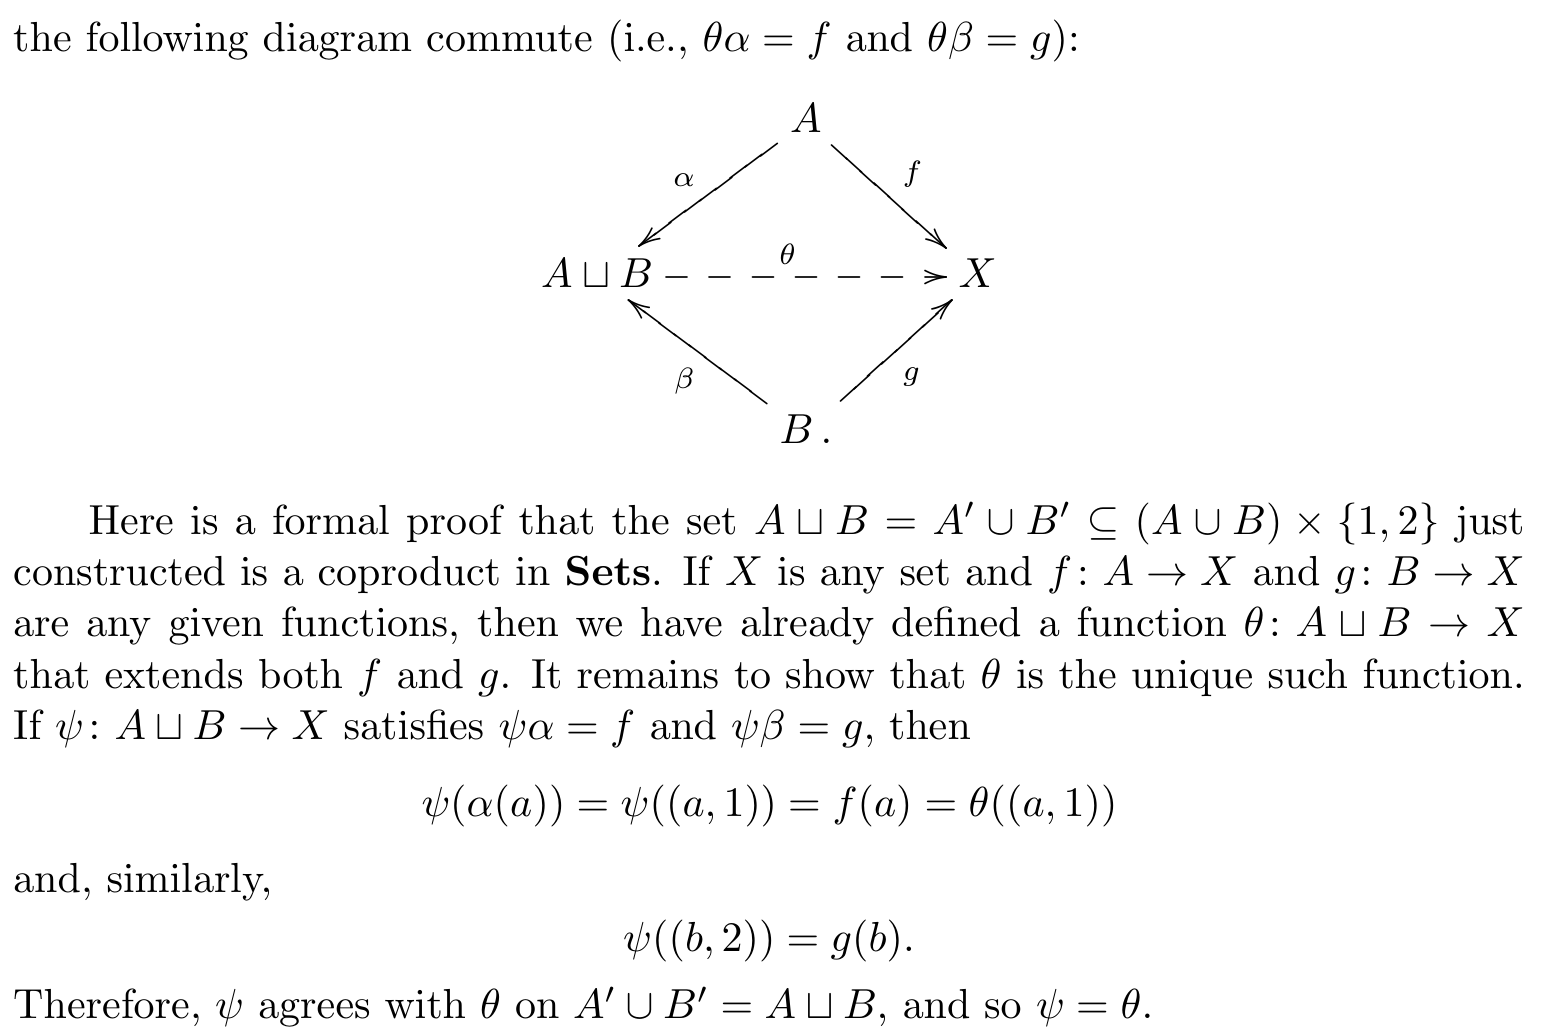
\includegraphics[width=\textwidth]{1-模范畴-2025052320.png}
% \caption{}
\label{}
\end{figure}

Coproduct does not always exists.

\begin{figure}[H]
\centering
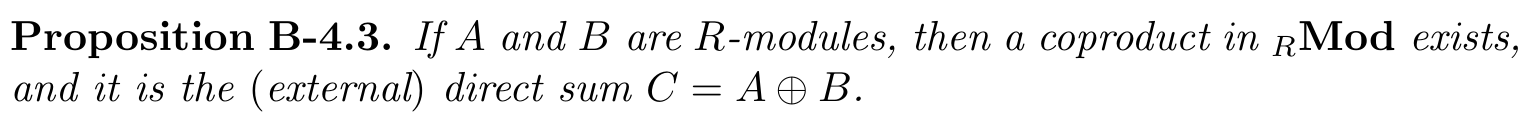
\includegraphics[width=\textwidth]{2-模范畴-2025052320.png}
% \caption{}
\label{}
\end{figure}

\begin{figure}[H]
\centering
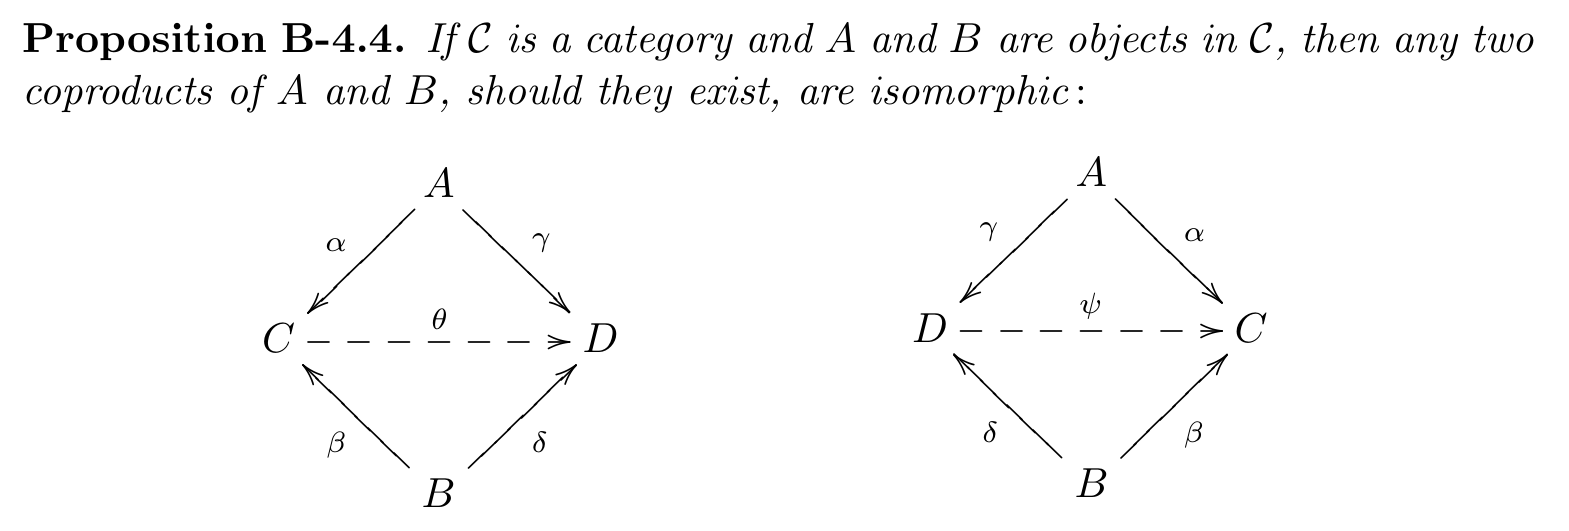
\includegraphics[width=\textwidth]{3-模范畴-2025052320.png}
% \caption{}
\label{}
\end{figure}

Here is a construction “dual” to coproduct.

\begin{figure}[H]
\centering
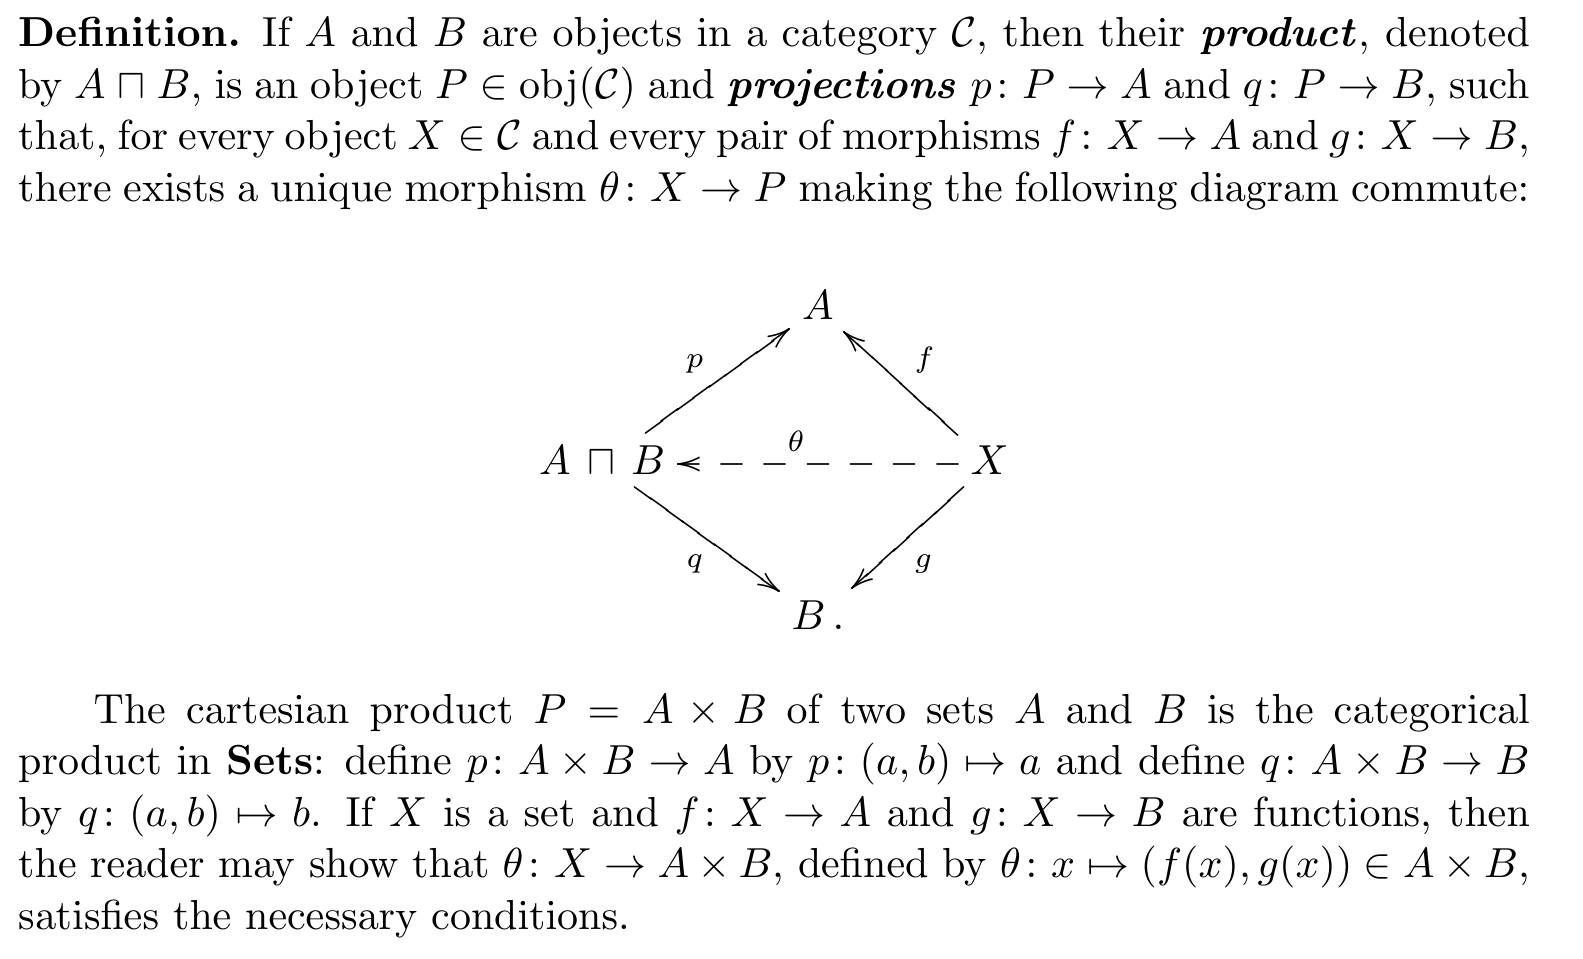
\includegraphics[width=\textwidth]{4-模范畴-2025052320.png}
% \caption{}
\label{}
\end{figure}

\begin{figure}[H]
\centering
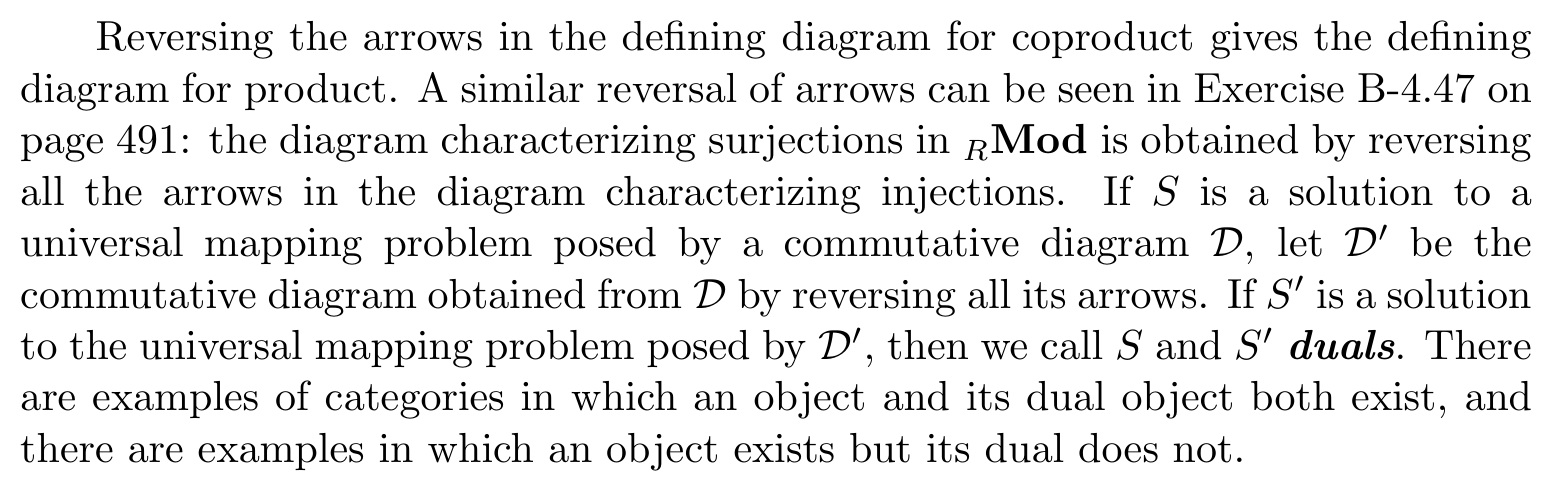
\includegraphics[width=\textwidth]{5-模范畴-2025052320.png}
% \caption{}
\label{}
\end{figure}

\subsection{Category applied to Hom between Module}

\begin{figure}[H]
\centering
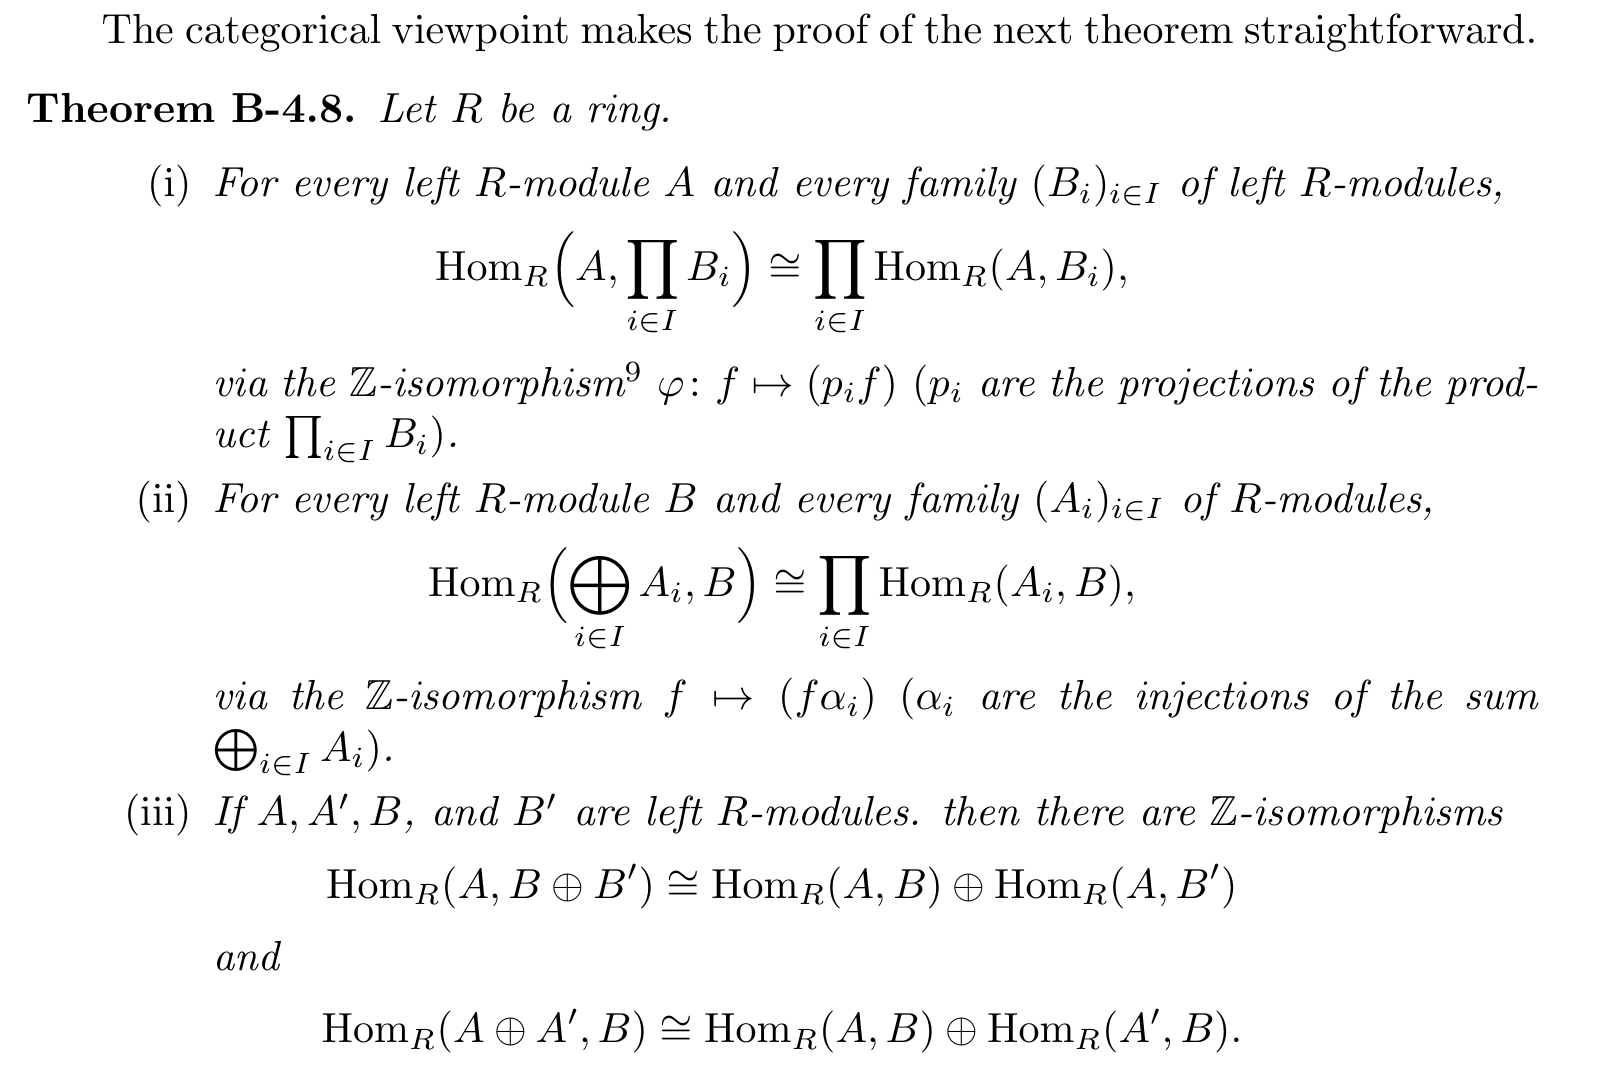
\includegraphics[width=\textwidth]{6-模范畴-2025052320.png}
% \caption{}
\label{}
\end{figure}

We show that $\varphi$ is both surjective and injective,

\begin{figure}[H]
\centering
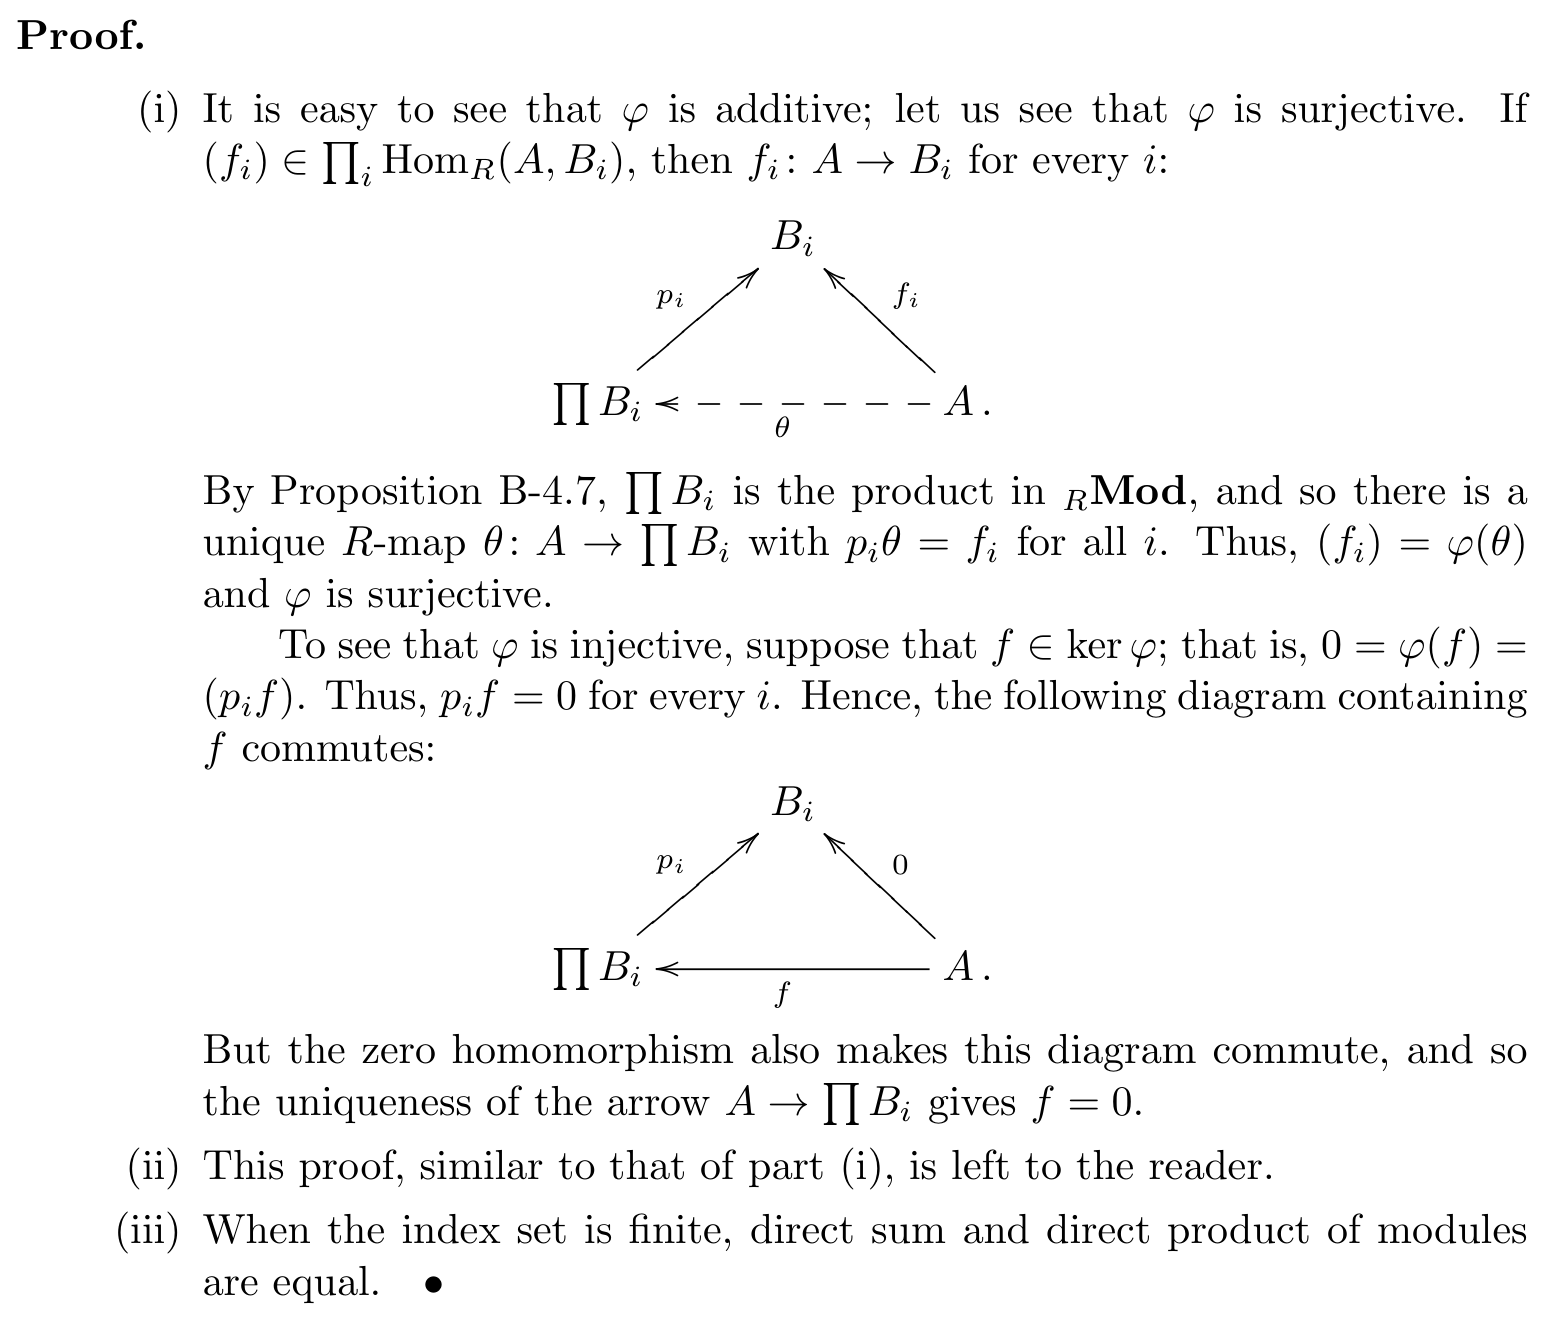
\includegraphics[width=\textwidth]{1-模范畴-2025052321.png}
% \caption{}
\label{}
\end{figure}

\subsection{Pullback and Pushout}

\begin{figure}[H]
\centering
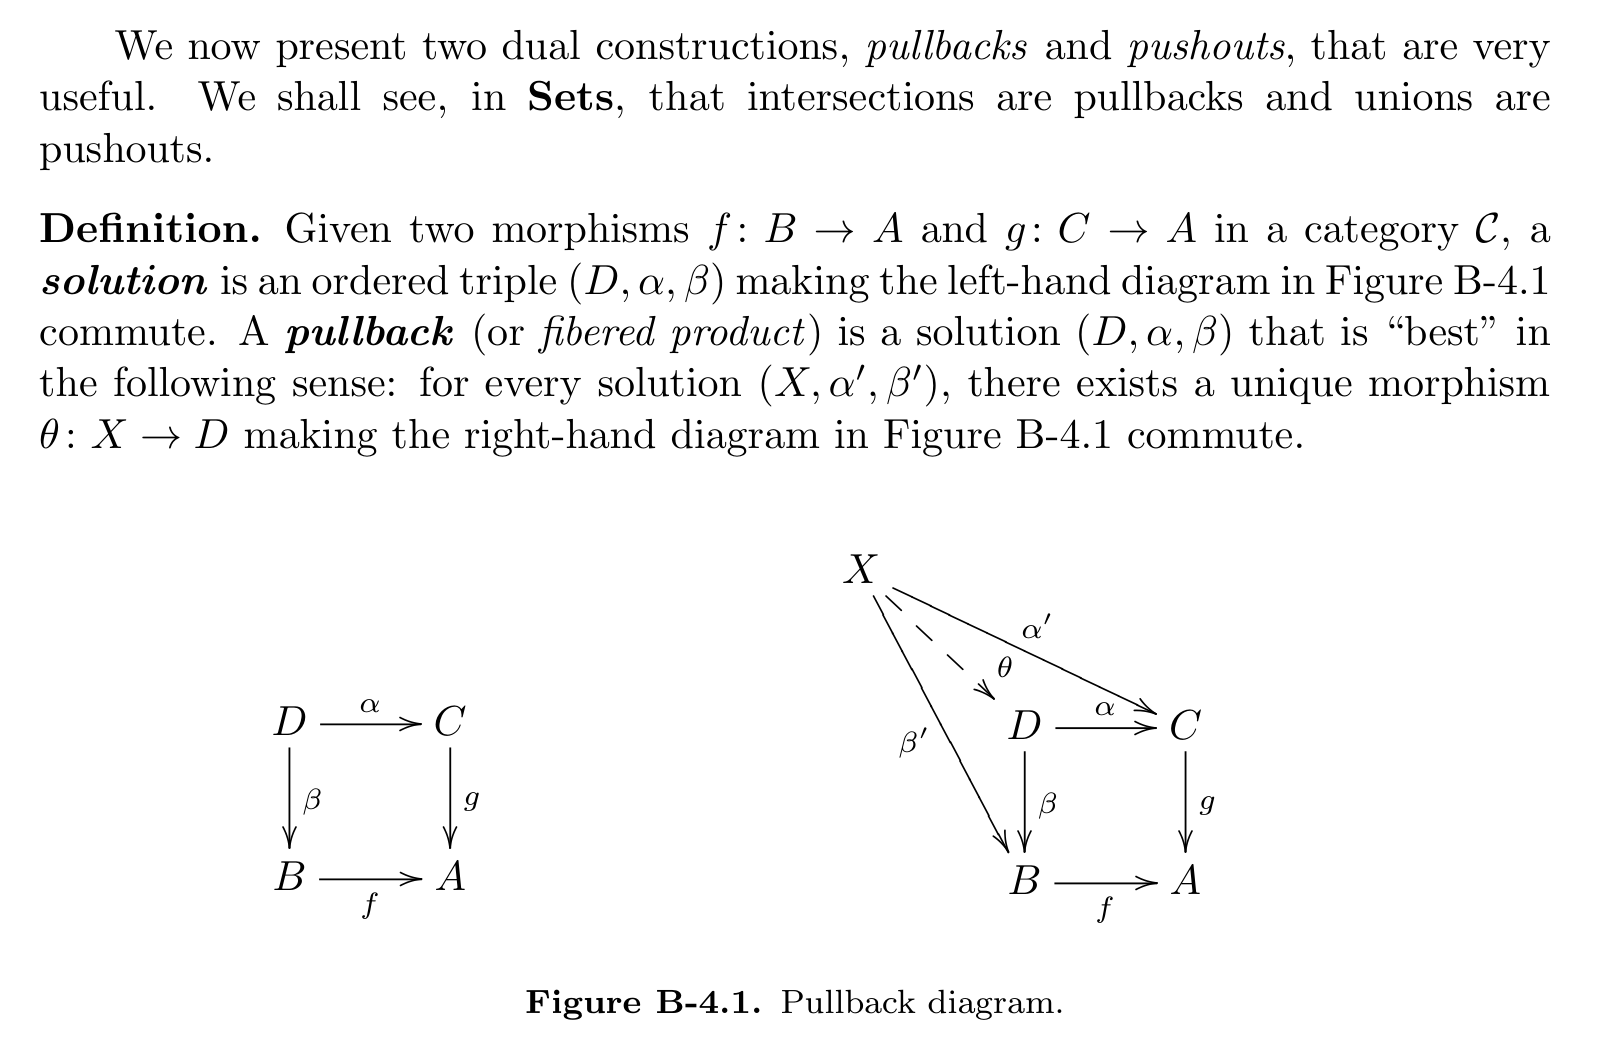
\includegraphics[width=\textwidth]{2-模范畴-2025052321.png}
% \caption{}
\label{}
\end{figure}

\subsubsection{Kernel as pullback}

\begin{figure}[H]
\centering
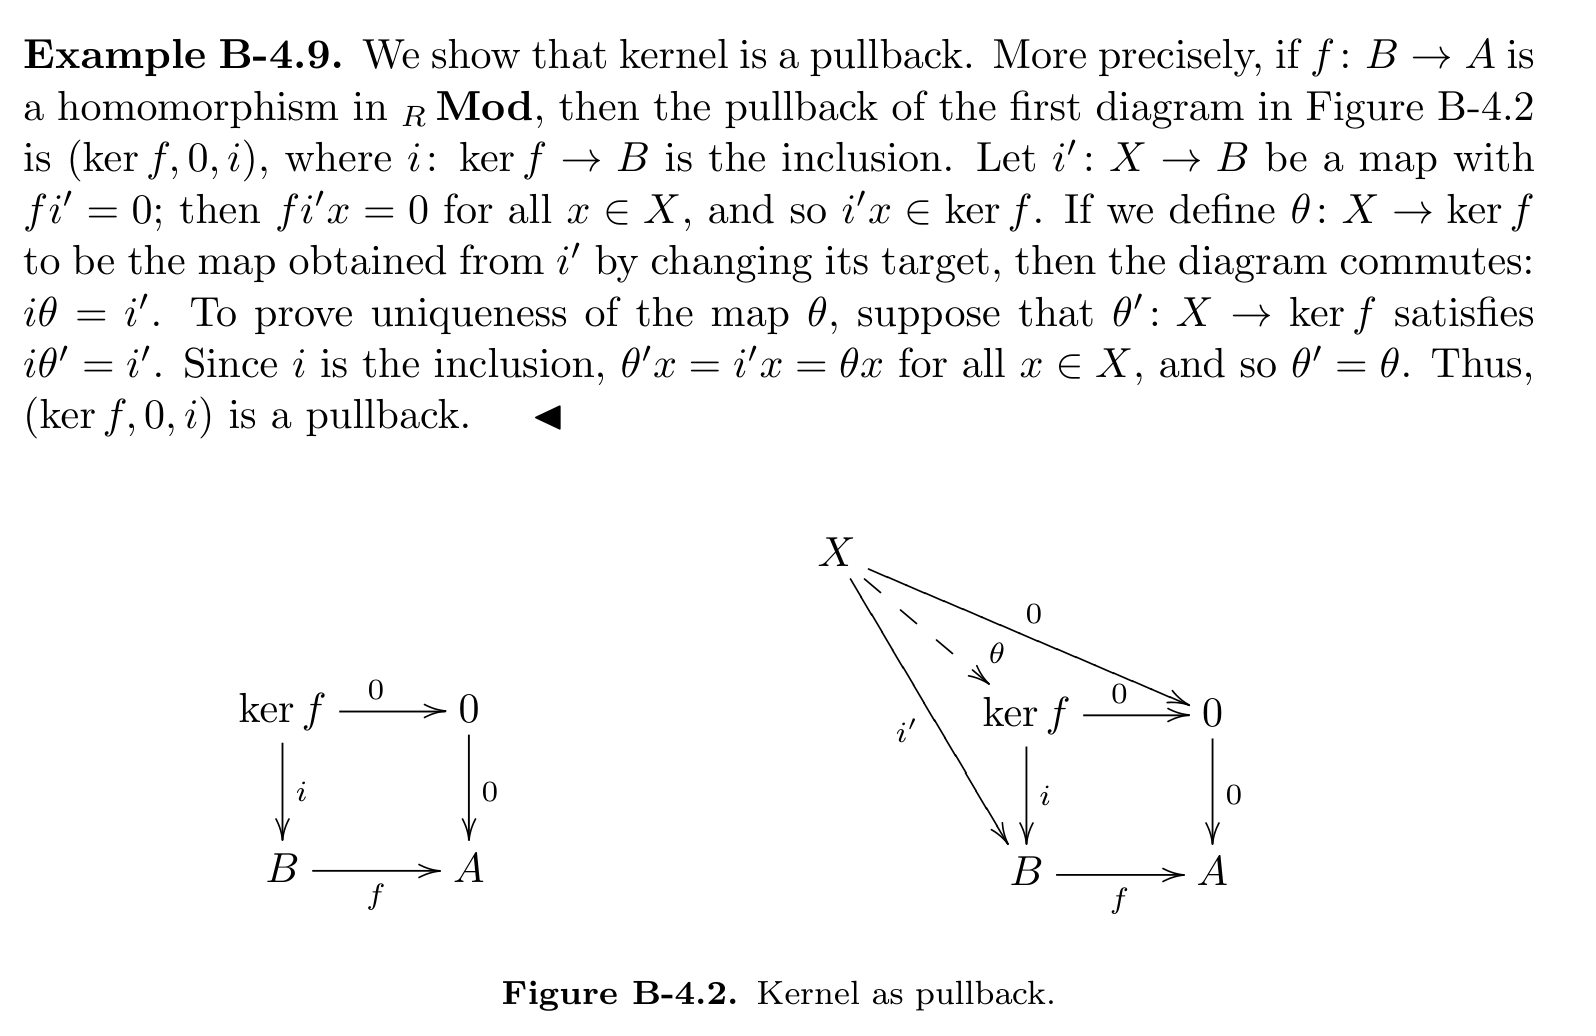
\includegraphics[width=\textwidth]{3-模范畴-2025052321.png}
% \caption{}
\label{}
\end{figure}

The key is that $i'x\in \ker f,\forall x\in X$; as $i$ is inclusion, we can construct a $\theta:X\to \ker f$ by mapping $x$ to $i'x$.
